\FloatBarrier
\subsection{Question 2}
In this section, we place our desired poles as shown in \autoref{code:pp21}. Our located poles does not cancell out the system zeros.  \autoref{fig:pp21} shows the step response of the closed loop system. Using the pulse input generated in last section, the system output and control signals are plotted at \autoref{fig:pp22}.

\begin{code}
	\begin{matlabcode}{firstnumber = 10}
	% Convert to state-space representation
	[A, B, C, D] = ssdata(Gz);
	
	% Check controllability
	Co = ctrb(A, B);
	if rank(Co) == size(A, 1)
	disp('System is controllable');
	else
	error('System is not controllable');
	end
	
	% Choose desired poles to improve settling time
	desired_poles = [0.4, 0.5, 0.8]; 
	
	K = place(A, B, desired_poles);
	
	sys_cl_no_kr = ss(A - B*K, B, C, D,sampleTimeIntervals);
	kr = 1 / dcgain(sys_cl_no_kr);
	
	% Create closed-loop system with precompensator
	B_cl = B * kr;
	sys_cl = ss(A - B*K, B_cl, C, D,sampleTimeIntervals);
	\end{matlabcode}
	\captionof{listing}{Pole placement without cancellation}
	\label{code:pp21}
\end{code}

\begin{figure}
	\centering
	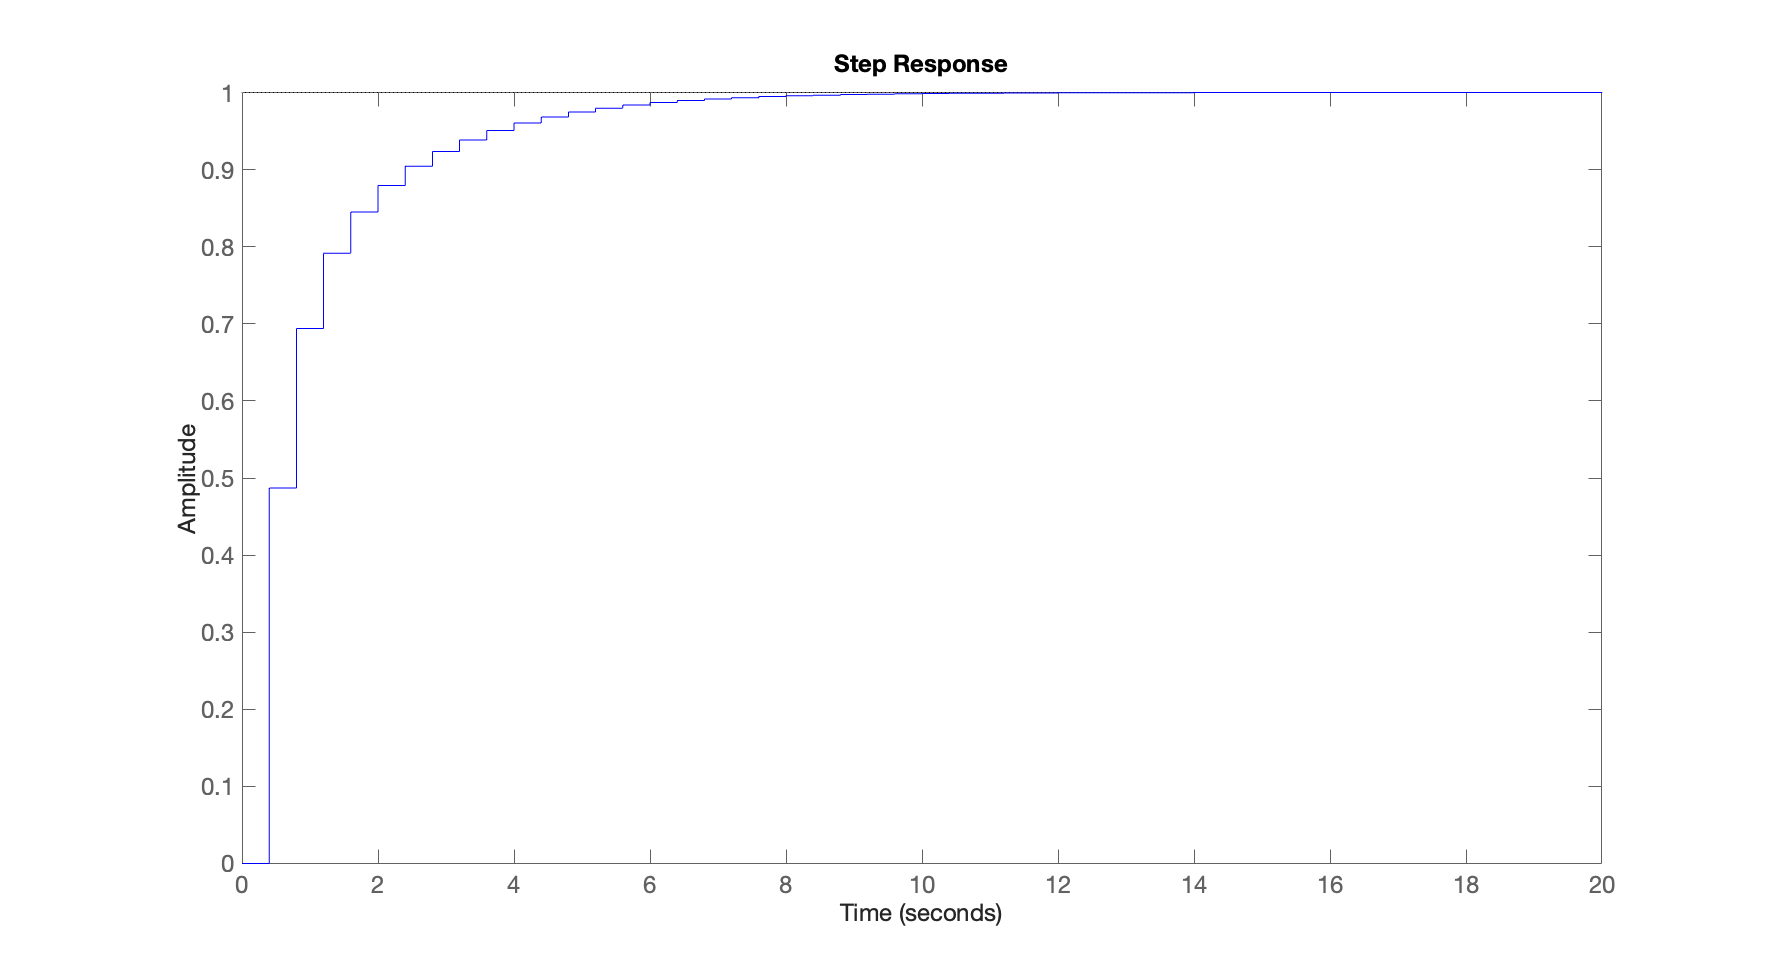
\includegraphics[width=\textwidth]{images/pp21.png}
	\caption{Step response of closed system without cancellation}
	\label{fig:pp21}
\end{figure}

\begin{figure}
	\centering
	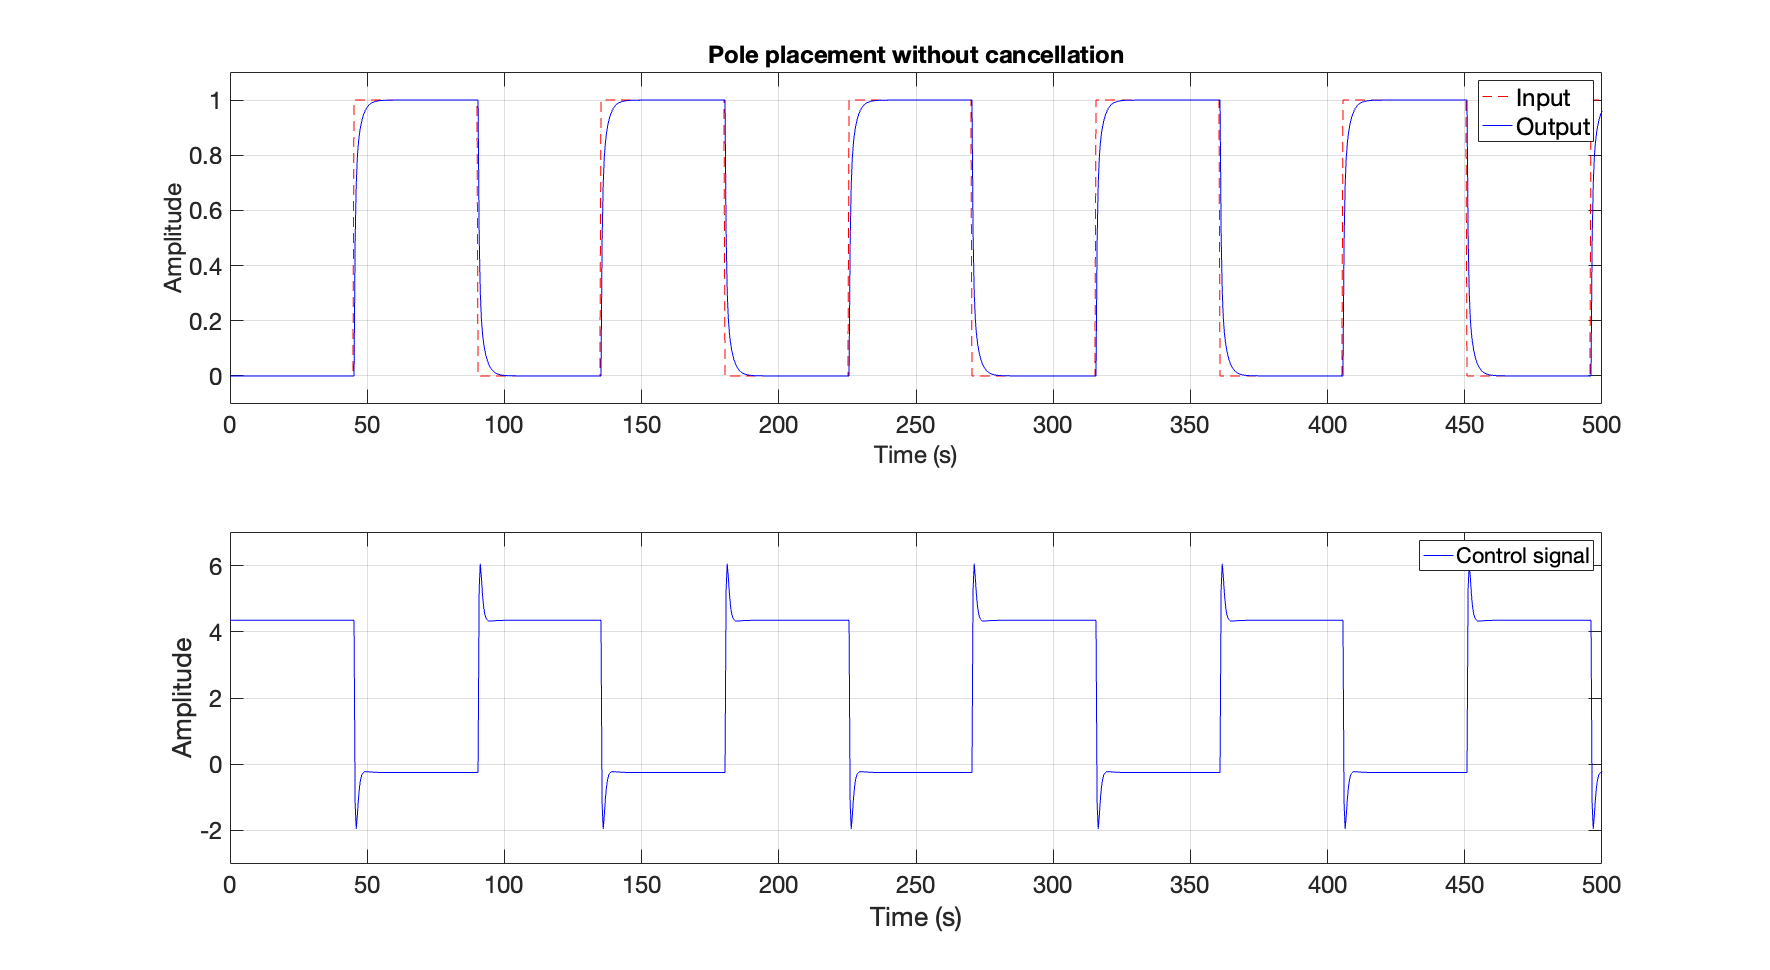
\includegraphics[width=\textwidth]{images/pp22.png}
	\caption{Pulse response of closed system without cancellation}
	\label{fig:pp22}
\end{figure}

The code  for this section is available at \lstinline|assignment2/part1/PP1_2.m|. 

